\section{Search}

Search may be used to search the application for any data that has been entered by a user. This ranges from the most basic data (the names used to display individual items within the display list) to more advanced queries involving relationships.

\begin{figure}[H]
\centering

\includegraphics[]{images/screenshots/search1.PNG}
\caption{Opening Search}
\label{fig:search_icon}
\end{figure}

To open search, click on the search icon located within the toolbar of the application as is outlined in red Figure~\ref{fig:search_icon} . Alternatively the shortcut keys Control/Command + F or Control + Space can be used to open the search dialog.

\begin{figure}[H]
\centering
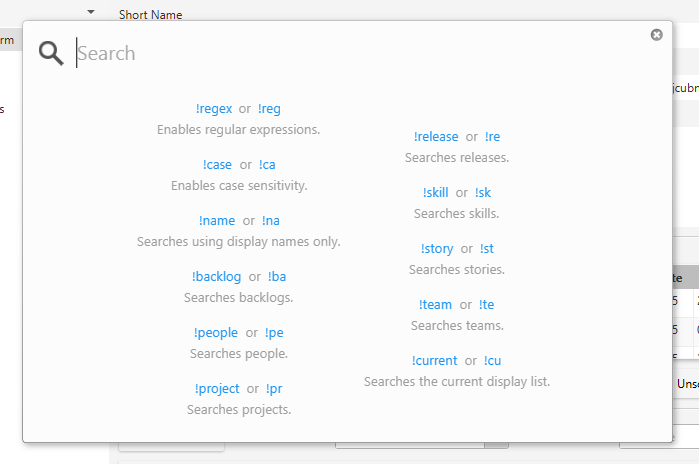
\includegraphics[width=\textwidth]{images/screenshots/search2.PNG}
\caption{Search Window}
\label{fig:search_window}
\end{figure}

Search will be presented in a window similar to the Figure~\ref{fig:search_window} . To begin a search immediately start typing and results will be shown as they are found.

Special search commands can be used in either their long or short versions to narrow or widen search criteria. They are global so can be typed anywhere within the search text and will apply to the entire query. Many can also be combined to perform a more specific or broad search.\newline
Other than by typing, search commands can be inserted from multiple places within the search window. These are from the screen that is first shown when opening search, the screen that is shown when there is no search query entered and this can also be shown by clicking the magnifying glass icon during a search. 

\begin{table}[h]
\centering
\caption{Special search commands}
\label{fig:search_commands}
\begin{tabular}{|c|c|l|}
{\bf Long Command} & {\bf Short Command} & {\bf Description}                                    \\
!current           & !cu                 & Searches the current display list only.              \\
!case              & !ca                 & Turns on case sensitivity.                           \\
!name              & !na                 & Searches display names only.                         \\
!regex             & !reg                & Turns on regular expressions \\
                   &                     &(instead of wildcards). \\
!backlog           & !ba                 & Searches backlogs.                                   \\
!people            & !pe                 & Searches people.                                     \\
!project           & !pr                 & Searches projects.                                   \\
!release           & !re                 & Searches releases.                                   \\
!skill             & !sk                 & Searches skills.                                     \\
!story             & !st                 & Searches stories.                                    \\
!sprint            & !sp                 & Searches sprints.                                    \\
!team              & !te                 & Searches teams.                                     
\end{tabular}
\end{table}

\begin{table}[H]
\centering
\caption{Special strings that can be entered as a part of a wildcard search.}
\label{fig:wildcard_commands}
\begin{tabular}{|c|l|}
{\bf Wildcard String} & {\bf Description} \\
\text{*}  &   Matches any series of characters. If \\
    &   unbounded will match from end of the \\
    &   current query to the end of any searched\\
    &   text.\\
?   &   Matches any single character.\\
\textbackslash \text{*} &   Matches a "\text{*}" character.\\
\textbackslash ? &   Matches a "?" character.
\end{tabular}
\end{table}

By default searches use wildcard expressions. These consist of a number of special strings that can be entered as a part of any normal search criteria.
Enabling regex mode (see special commands above) {\bf disables wildcards} and {\it instead all search terms are treated as regular expressions.}\newline


Complex expressions using "\&\&" and "\text{\textbar}\text{\textbar}" can be constructed at anytime within search. "\&\&" is used to represent a logical "and" (both left and right sides must be met). "\text{\textbar}\text{\textbar}" is used to represent a logical "or" (either the left side, the right side or both must be met).\newline
Standard order of operations applies, with "\&\&" having a higher precedence than "\text{\textbar}\text{\textbar}". These operators work with any of the special commands defined above.\newline
{\bf At this time we do not support brackets in our complex expressions} instead they will be treated as part of the search query.

\begin{figure}[H]
\centering
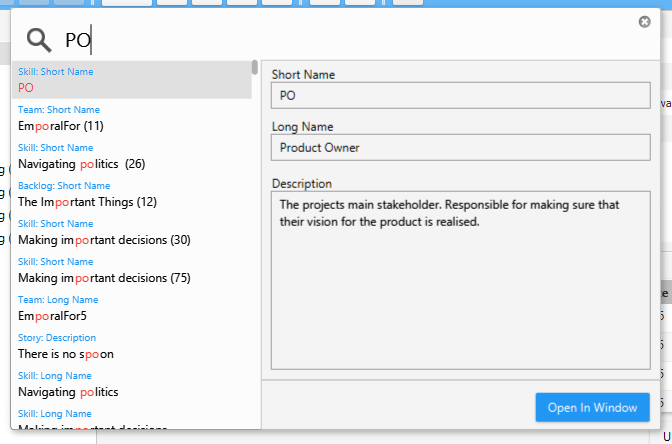
\includegraphics[width=\textwidth]{images/screenshots/search3.PNG}
\caption{Search window with results}
\label{fig:search_window_results}
\end{figure}

When the search results window has results, hovering over each item either with the mouse or the arrow keys will render a preview in the right-hand pane. Clicking on the "Open In Window" button of the preview, clicking on the search result or pressing the enter/return key on the keyboard will take you to the search result in your current window.

The search results window can safely be closed and re-opened during a search as search results will persist between openings of this window.